\documentclass{article}

% --- load packages ---
\usepackage[margin=1in]{geometry} % change the margins
\usepackage{amsmath} % useful math environments and commands like align
\usepackage[colorlinks,bookmarks,bookmarksnumbered,allcolors=blue]{hyperref} % hyperlinks between references
\usepackage{graphicx}  % include images
\usepackage[table,xcdraw]{xcolor}
\usepackage[caption=false]{subfig} % subfigures.  false option prevents conflicts in caption styling with other packages
\usepackage{booktabs} % better tables
\usepackage[capitalise]{cleveref} % better referencing. uses cref.
\usepackage[section]{placeins} % sometimes useful to prevent figures from floating out of a section
\usepackage{cite} % handles multiple citations in one command better
\usepackage{doi} % allow correct hypderlinking of DOIs
\usepackage[normalem]{ulem}
\usepackage{float}
\usepackage{minted}
\usepackage{pdfpages}
\usepackage{tikz}
\usetikzlibrary{tikzmark}


%\usepackage{lmodern}

\useunder{\uline}{\ul}{}


\begin{document}

\title{Optimal Spring Sizing}
\author{Landon Wright}
% put in \date{} if you don't want a date to appear, or enter a specific date, otherwise default is today's date.
\maketitle
\begin{centering}
\section{Summary}

\end{centering}
\subsection{Design variable values}
The optimal cost was found to be \textbf{\$400,140}.
The determined optimum values for the design variables are as follows:

\begin{table}[H]
\centering
\caption{Optimum values for design}
\label{tab:optimum values}
\begin{tabular}{ll}
\hline
\textbf{Variable}      & \textbf{Value} \\
\hline
Velocity & $7.8161 \frac{ft}{s}$ \\
Pipe Diameter & $0.1816 ft$ \\
Particle Size  & $0.0005 ft$    \\
Water Flow Rate   & $0.1128 \frac{ft^{3}}{s}$\\
Volumetric Concentration & $0.4$\\
Slurry Density & $104.84 \frac{lbm}{ft^{3}}$\\

\hline

\end{tabular}
\end{table}
\newpage

\section{Procedure}
\subsection{Equation Sequence}
\begin{center}
	\begin{tabular}{|l|l|}
		\hline
		Get values from optimizer (V, D, d) & Optimization code will set these variables \\ 
		\hline
		$Q = \pi * \frac{D^{2}}{4} * V$ & Volumetric flow rate \\ 
		\hline
		$Q_{l} = \frac{W}{\rho_{l}}$ & Lime volumetric flow rate \\ 
		\hline
		$Q_{w} = Q - Q_{l}$ & Water volumetric flow rate \\ 
		\hline
		$c = \frac{Q_{l}}{Q}$ & Volumetric concentration \\ 
		\hline
		$\rho = \rho_{w} + c * (\gamma - \rho_{w})$ & Slurry density \\ 
		\hline
		$C_{d}R_{p}^{2} = 4  g  \rho_{w}  d^{3}\left ( \frac{\gamma - \rho_{w}}{3\mu^{2}}\right )$ & Eqn (3) \\ 
		\hline
		$C_{d} = e^{-0.001 log(C_{d}R_{p}^{2})^3 + 0.0583 log(C_{d}R_{p}^{2})^2 - 1.1497 log(C_{d}R_{p}^{2}) + 6.4442}$ & Fit of empirical data \\ 
		\hline
		$R_w = \frac{\rho_w V D}{\mu}$ & Reynolds number \\ 
		\hline
		$\left\{\begin{matrix}f_w = \frac{0.3164}{R_w^{0.25}} \text{ \: if \:} R_w \leq 10^5\\f_w = 0.0032+0.221R_w^{-0.2377}\end{matrix}\right.$ & Water friction factor \\ 
		\hline
		$f = f_w \left [\frac{\rho_w}{\rho} + 150 c \frac{\rho_w}{\rho}\left (\frac{g D (S -1)}{V^2 \sqrt{C_d}} \right )^{1.5} \right ]$ & Friction factor \\ 
		\hline
		$\delta p = \frac{f \rho L V^2}{D 2 g_c}$  & Pressure loss due to friction \\
		\hline 
		$P_p = \delta p * Q$& Pump power required \\ 
		\hline
		$P_g = 218 W \left ( \frac{1}{\sqrt{d}} - \frac{1}{\sqrt{a}} \right )$& Power grind required \\ 
		\hline
		$HP_p = \frac{P_g}{550}$& Horsepower to pump  \\ 
		\hline
		$HP_g = \frac{P_g}{550}$& Horsepower to grind \\ 
		\hline
		$C_p = 300 HP_g + 200 HP_g$& Purchase cost of system \\ 
		\hline
		$C_o = (0.07 HP_g + 0.05 HP_p) * 8 * 300 *\left ( \frac{1.07^7 - 1}{0.07 * 1.07^7} \right)$& Operational cost of system \\ 
		\hline
		$C = C_p + C_o$& Total system cost \\ 
		\hline
		
	\end{tabular} 
\end{center}
\subsection{Mapping Table}
\begin{center}
	\begin{tabular}{|l|l|}
		\hline
		\textbf{Variables}                       & \textbf{Design Variables}                \\
		Average flow velocity (V) \tikzmark{a}   & \tikzmark{d} Average flow velocity (V)   \\
		Internal pipe diameter (D) \tikzmark{b}  & \tikzmark{e}Internal pipe diameter (D)               \\
		Average particle size after grinding (d)\tikzmark{c} & \tikzmark{f}Average particle size after grinding (d) \\
		length of pipeline (w)                   &                                          \\
		Limestone flowrate (W)                   &                                          \\
		Average lump size before grinding (a)    &                                          \\
		Gravity (g)                              &                                          \\
		Density of water ($\rho_w$)              &                                          \\
		Viscosity of water ($\mu$)               &                                          \\
		Limestone density ($\gamma$)             &                                          \\
		\hline
		\textbf{Analysis Functions}              & \textbf{Design Functions}                \\
		Volumetric slurry concentration (c)      & \tikzmark{i}Minimize cost                \\
		Water flow rate ($Q_w$)                  &  s.t.                                    \\
		Density of slurry ($\rho$)               &  \tikzmark{j}$V \geq 1.1 * V\_c$         \\
		Limestone flowrate (volumetric) ($Q_l$)  &                                          \\
		Slurry flow rate (Q)                     &                                          \\
		Grinding Power ($P_g$)                   &                                          \\
		Friction factor (f)                      &                                          \\
		Water friction factor ($f_w$)            &                                          \\
		Average drag coefficient ($C_d$)         &                                          \\
		Limestone specific gravity (S)           &                                          \\
		Reynolds number ($R_w$)                  &                                          \\
		$C_dR_p$                                 &                                          \\
		Slurry density ($\rho$)                  &                                          \\
		Pipe pressure drop ($\delta p$)          &                                          \\
		Pumping power ($P_f$)                    &                                          \\
		Critical velocity ($V_c$) \tikzmark{g}   &                                          \\
		Cost (C) \tikzmark{h}                    &                                          \\
		\hline
	\end{tabular}
	\begin{tikzpicture}[overlay, remember picture, yshift=.25\baselineskip, shorten >=.5pt, shorten <=.5pt]
		\draw [->] ([yshift=3pt]{pic cs:a}) to ([yshift=3pt]{pic cs:d});
		\draw [->] ([yshift=3pt]{pic cs:b}) to ([yshift=3pt]{pic cs:e});
		\draw [->] ([yshift=3pt]{pic cs:c}) to ([yshift=3pt]{pic cs:f});
		\draw [->] ([yshift=3pt]{pic cs:h}) to ([yshift=3pt]{pic cs:i});
		\draw [->] ([yshift=3pt]{pic cs:g}) to ([yshift=3pt]{pic cs:j});
	\end{tikzpicture}
	
\end{center}
\subsection{Model Validation}
The curve fit was performed in the statistical package JMP. It is a third order fit of the log of both $C_d$ and $C_dR_p^2$ data that was provided in the problem statement.  The $R^2$ value of the fit is exceptionally high at 0.9999 which suggests that the data is very well approximated by the fit.


\section{Results and Discussion}
\subsection{Optimum Values}
\begin{center}
\begin{tabular}{|l|l|}
	\hline
	\textbf{Variable/Function}               & \textbf{Value at optimum} \\
	Average flow velocity (V)                & 7.2599                    \\
	Internal pipe diameter (D)               & 0.1816                    \\
	\cellcolor{yellow}Average particle size after grinding (d) & 0.0005                    \\
	length of pipeline (w)                   & 79200                     \\
	Limestone flowrate (W)                   & 12.67                     \\
	Average lump size before grinding (a)    & 0.01                      \\
	Gravity (g)                              & 32.17                     \\
	Density of water ($\rho_w$)              & 62.4                      \\
	Viscosity of water ($\mu$)               & 0.0007392                 \\
	Limestone density ($\gamma$)             & 168.5                     \\
	\cellcolor{yellow}Volumetric slurry concentration (c)      & 0.4                       \\
	Water flow rate ($Q_w$)                  & 0.1128                    \\
	Density of slurry ($\rho$)               & 104.84                    \\
	Limestone flowrate (volumetric) ($Q_l$)  & 0.0752                    \\
	Slurry flow rate (Q)                     & 0.188                     \\
	Grinding Power ($P_g$)                   & 95902                     \\
	Friction factor (f)                      & 0.0175                    \\
	Water friction factor ($f_w$)            & 0.0173                    \\
	Average drag coefficient ($C_d$)         & 13.3093                   \\
	Limestone specific gravity (S)           & 2.7003                    \\
	Reynolds number ($R_w$)                  & 111280                    \\
	$C_dR_p$                                 & 64.9645                   \\
	Pipe pressure drop ($\delta p$)          & 656410                    \\
	Pumping power ($P_f$)                    & 123390                    \\
	Critical velocity ($V_c$)                & 6.5999                    \\
	Pumping HP ($HP_p$)						 & 224.35					 \\
	Grinding HP ($HP_g$)					 & 174.37					 \\
	Cost (C)                                 & 400140                    \\
	\hline
\end{tabular}
\end{center}
\subsection{Optimum and Design Space}
A slice of the design space is shown in figure \ref{fig:plotzoomed}.  As can be seen in the figure the feasible design space is rather small in comparison to the total design space. It occupies a small triangular section of the space and shows that the optimum is heavily constrained. The optimum, marked with a red star in the figure is a constrained optimum and could be enhanced by relaxing the constraints on the volumetric concentration and the critical velocity, however it is unlikely that these constraints can be relaxed as they are governed by physical phenomena.  The constraint is most likely a global optimum of the design space due to the somewhat simple nature of the contour lines.

\subsection{Contour Plot}
\begin{figure}[H]
	\centering
	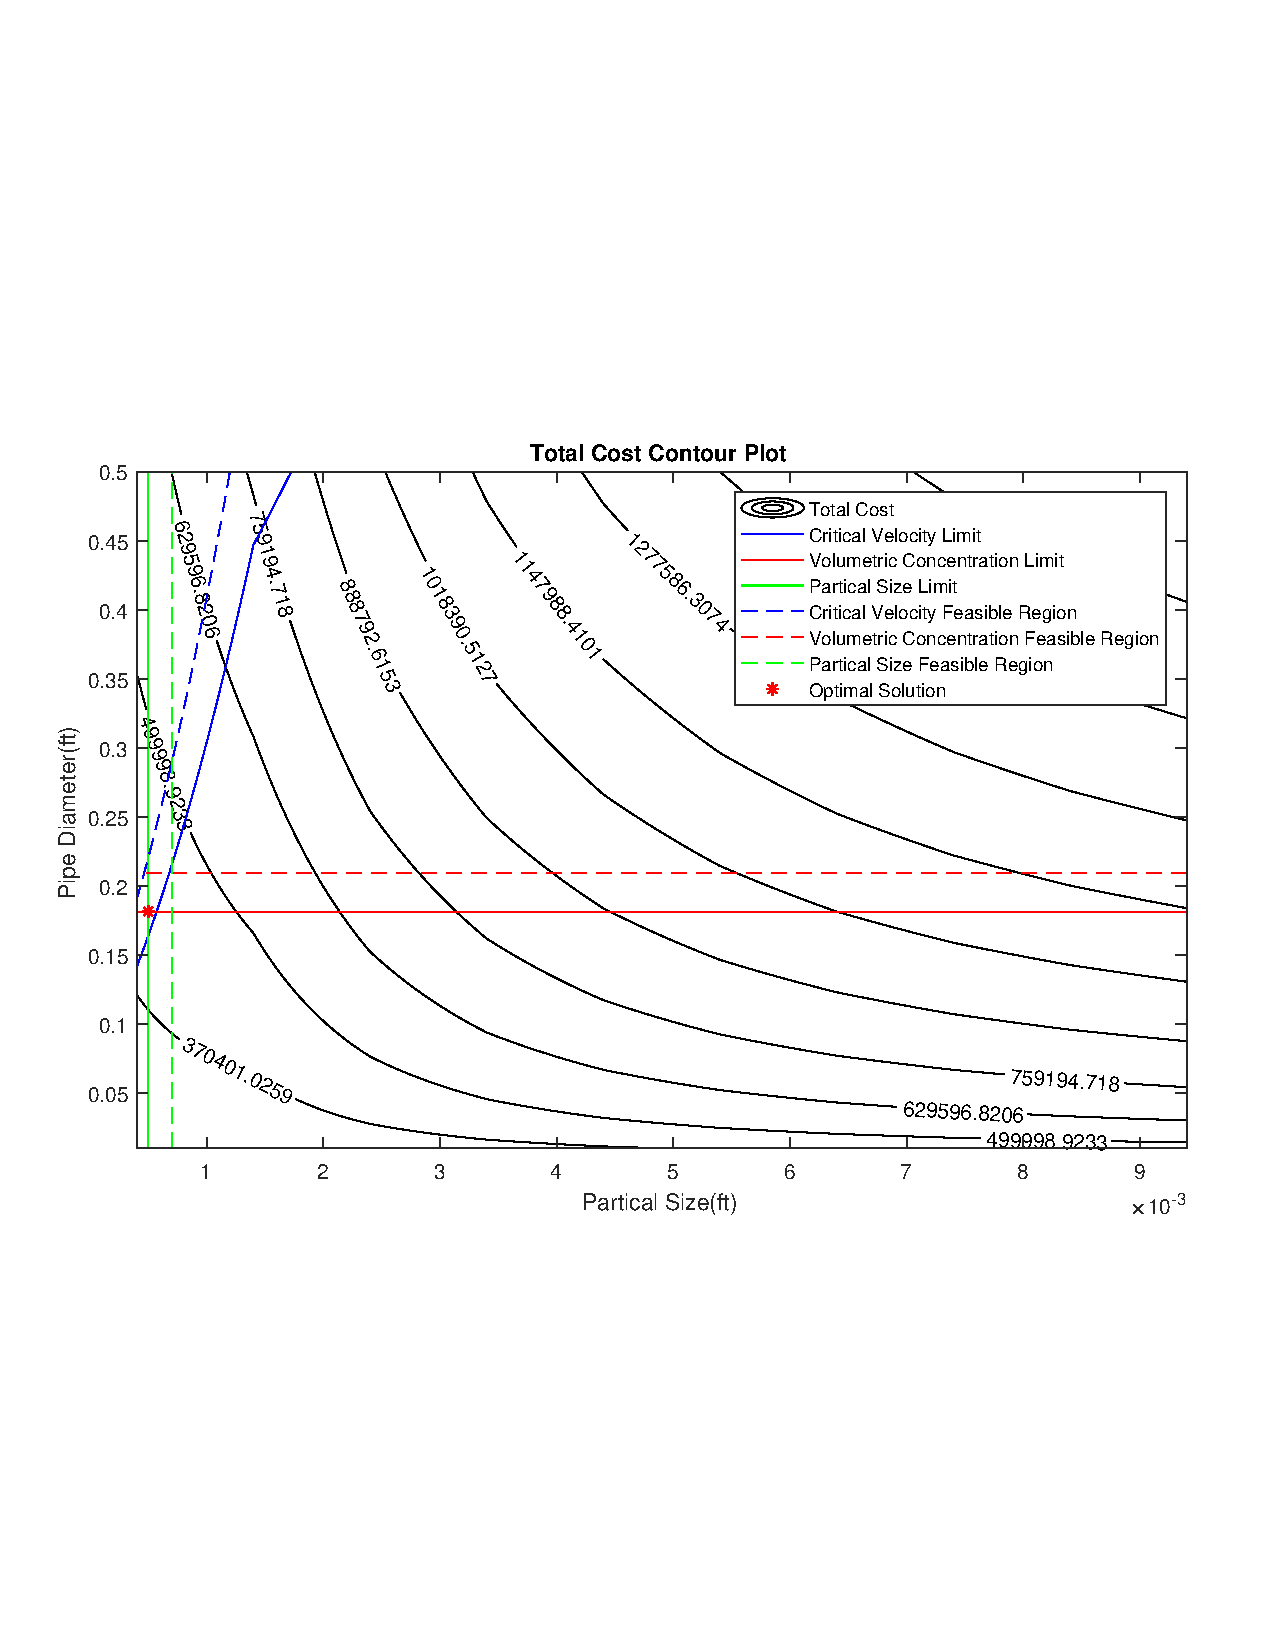
\includegraphics[width=0.9\linewidth]{PlotBig}
	\caption{Plot of the design space}
	\label{fig:plotzoomed}
\end{figure}

\subsection{Other Observations}
It is of interest that this model is constrained so tightly considering the relatively few number of constraints that exist in the problem, however all of the constraints shown in figure \ref{fig:plotzoomed} contribute to constraining the optimum value of the problem.  As mentioned above the optimum could be enhanced through the relaxation of the critical velocity and volumetric concentration limits, however this would likely lead to clogging issues in the system and is not recommendable.  It is also important to not that this contour plot only shows three (two varied with one held constant) of a total 6 possible dimensions of the problem.  To further understand the design space it would be necessary to create several similar plots of the other variables.

\section{Appendix}

\subsection{Matlab files}
\subsubsection{Optmization code}
\inputminted[xleftmargin=20pt,linenos]{matlab}{Opt.m}
\subsubsection{ObjCon Function}
\inputminted[xleftmargin=20pt,linenos]{matlab}{objcon.m}
\subsubsection{Plotting Code}
\inputminted[xleftmargin=20pt,linenos]{matlab}{contourPlot.m}

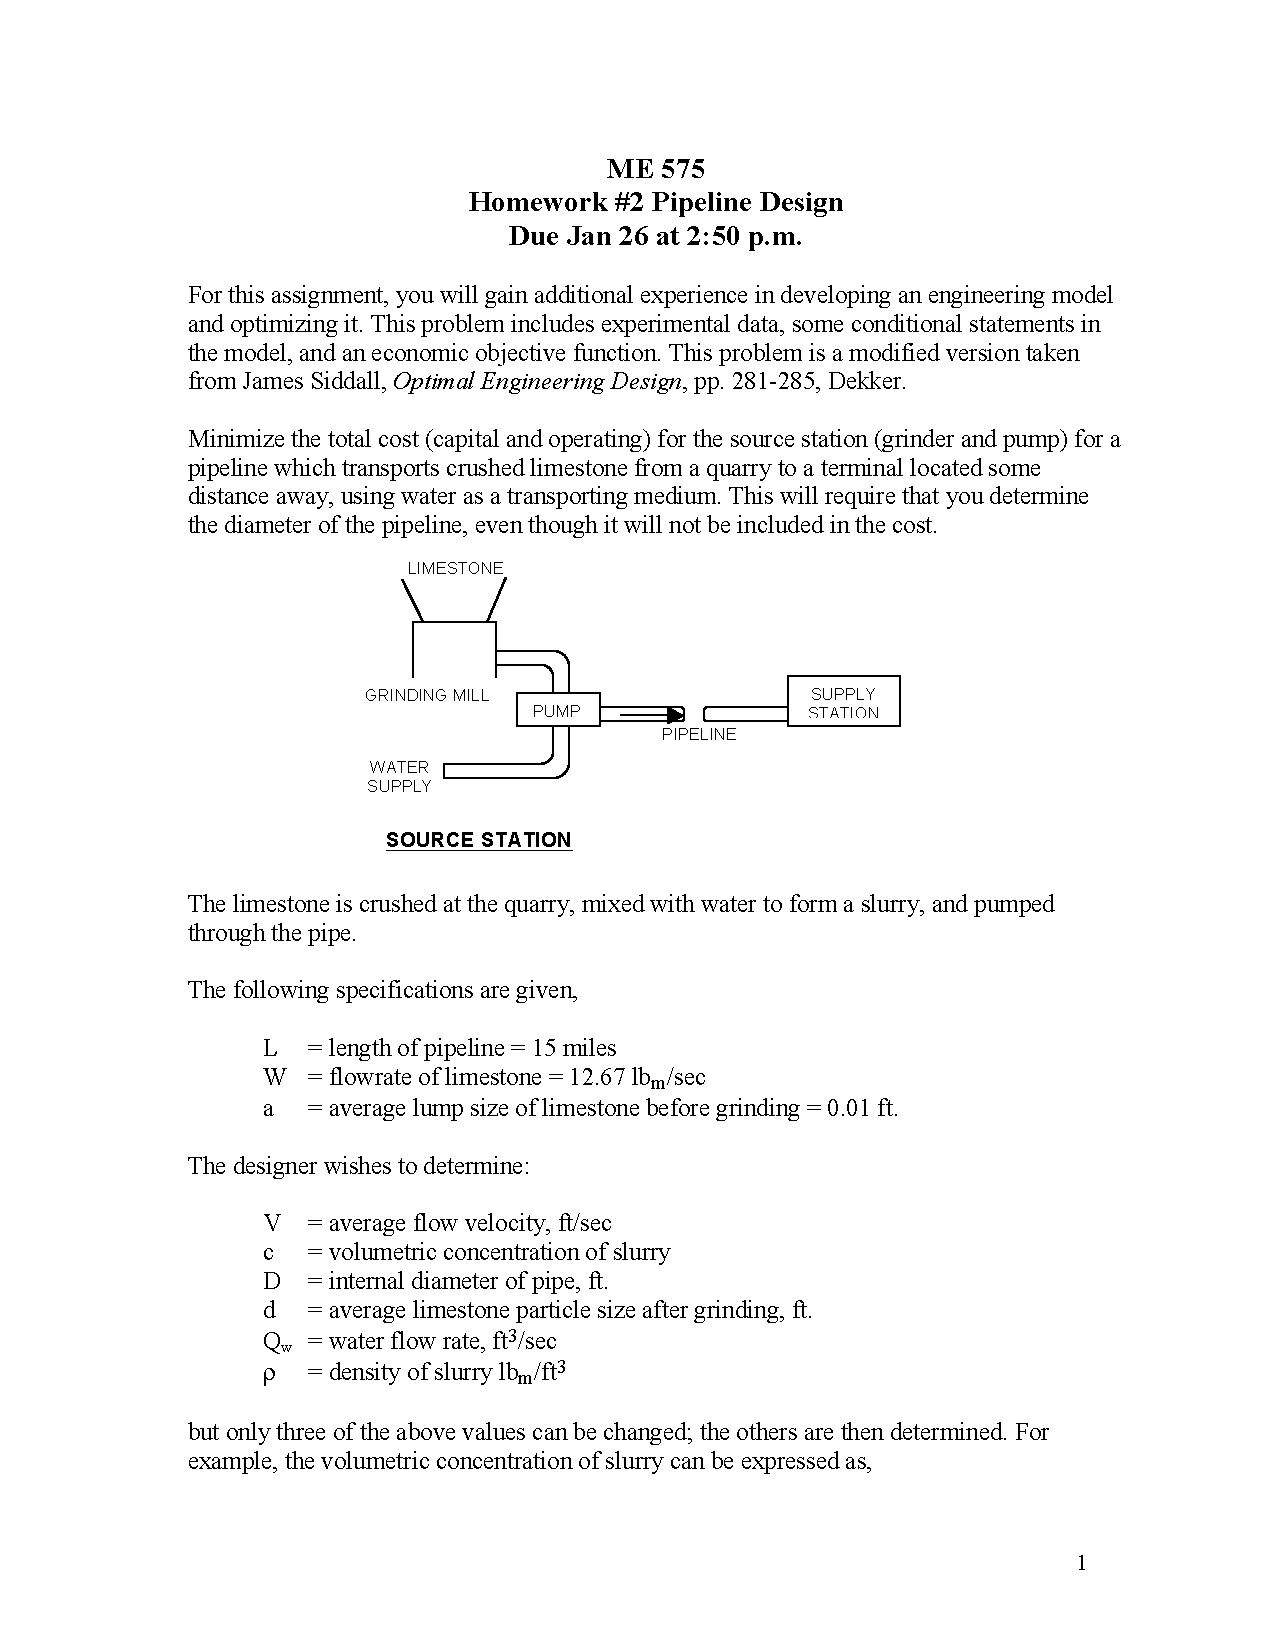
\includepdf[pages=-, pagecommand={}]{HW2Slurry.pdf}
\end{document}